\chapter{声色見本帳}
\thispagestyle{myheadings}

本研究で提案するサービス「声色見本帳」は,ユーザが求める声の評価スコアを入力し,その評価スコアに近い合成音声ライブラリを探索・提案するサービスである.
ユーザは自身が求める声に近いライブラリを,多くのライブラリの声を手探りで聞き比べる手間なく自身に合った声を探索できる.
ライブラリの作成者も,自身のライブラリを多くのユーザに知ってもらう機会を得られる.
実際に作成したサービスの画面を図\ref{fig:site_image}に示す.

\begin{figure}[h]
  \centering
  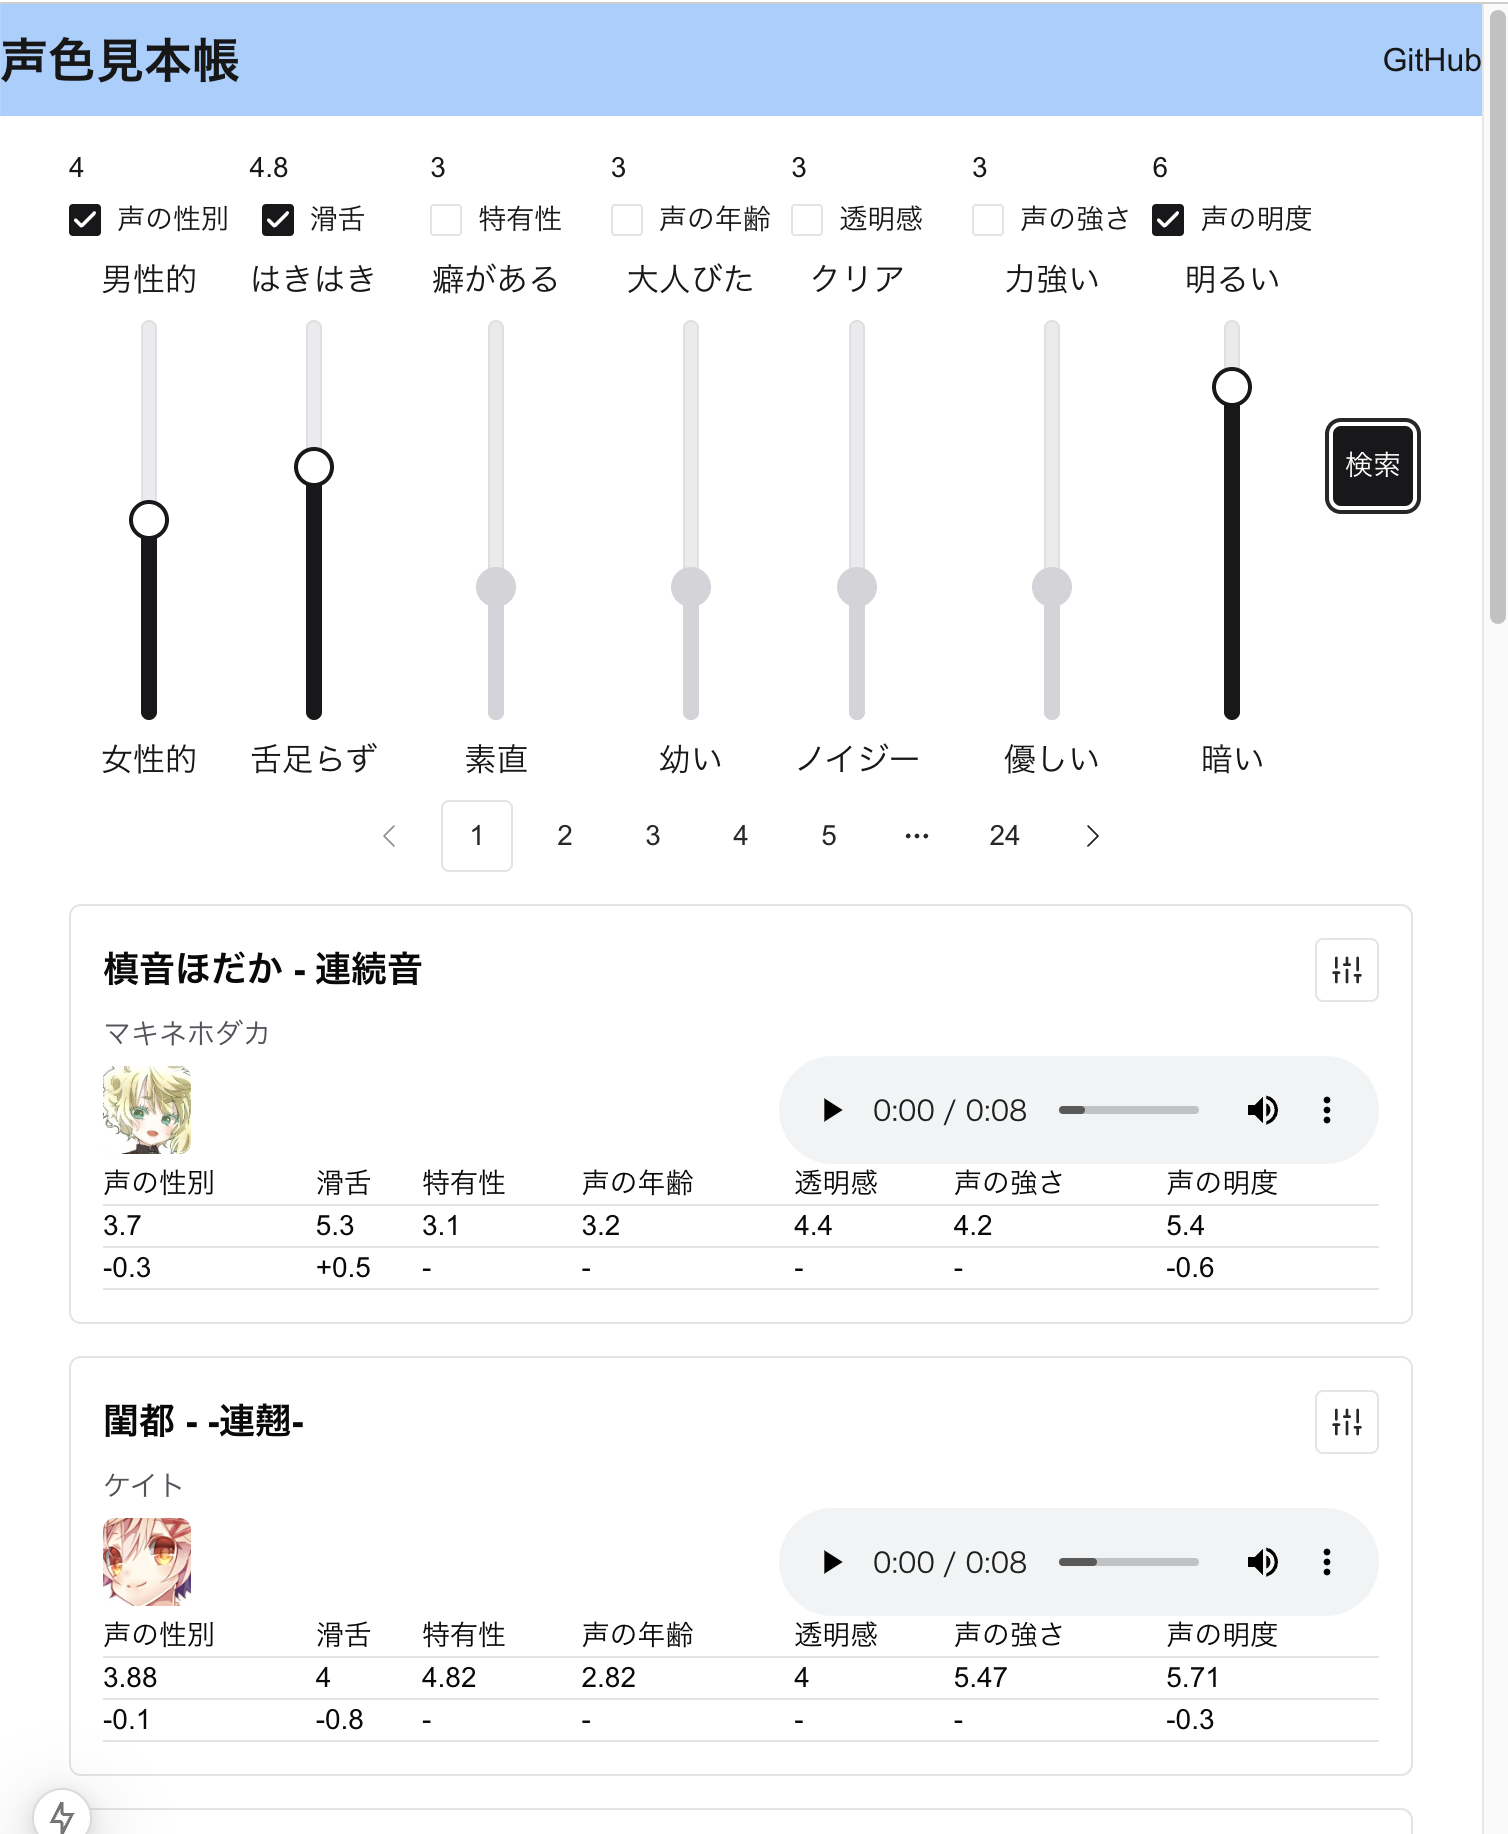
\includegraphics[width=0.9\linewidth]{fig/site_image.png}
  \caption{サービスの画面イメージ}
  \label{fig:site_image}
\end{figure}

\section{要求仕様}

本研究で提案するサービスについての要求仕様を以下に示す.
ユーザは求める声の評価スコアを数値として入力し,その評価スコアに近いUTAU音源ライブラリを探索できる.
探索結果として提示されたライブラリの歌声を実際に聞ける機能も必要である.
評価スコアを用いて声質を表現できるとしても,実際に聞いてみて本当に入力した評価スコアが求める声に近いかを確認したり,探索結果として提示されたライブラリの中から好みの声を選べる.
探索結果からは配布ページへのリンクを確認でき,ユーザがスムーズにライブラリをダウンロードできる.
また,ユーザが新しいライブラリを追加できる機能も提供する.
追加されたライブラリはサービスに登録されると同時に評価スコアが自動で推定され,以降の探索対象として利用される.
この機能により,サービスに登録されていなかったライブラリや,今後公開されるライブラリも将来的に探索できる.
サービスはWebサービスとして実装し,ユーザがブラウザから手軽に利用できるかたちにする.
合成音声ソフトウェアであるUTAUはスマートフォンではなくPCでの利用が一般的であるため,そのライブラリの探索もPCで行うのが自然である.
よってサービスはPCでの利用を前提としてデザインを行う.

\section{実装}
サービスのフロントエンドはTypeScriptを用いて開発し,フレームワークとしてNext.js,UIコンポーネントライブラリとしてChakra UIを用いて実装した.
バックエンドはPythonを用いて開発し,フレームワークとしてFastAPIを,データベースとしてはPostgreSQLを用いて実装した.
バックエンドをPythonで実装したため,ライブラリを追加する際事前に構築した機械学習モデルによる推論やサンプル音声の合成を一挙に行える.

\subsection{ライブラリ探索機能}

探索はサービスのトップ画面から行う.
ユーザは求める声の評価スコアを7つの評価軸に対してスライダーを用いて評価スコアを0.1刻みの小数で入力した後,探索ボタンをクリックして探索を行う.
スライダーによる入力インタフェースに加えそのスライダーの両端に評価スコアの高低に対応する表現語を配置したため,数値である評価スコアと表現語の表す声との関係を直感的に理解できる.
探索ボタンをクリックするとAPIを通じてデータベースにアクセスし,入力された評価スコアに近いライブラリを探索し,その結果をユーザに提示する.

入力の際,ユーザは各評価軸ごとに存在するチェックボックスを操作できる.
チェックボックスはデフォルトでは全てチェックされており,チェックを外すと対応する評価軸を無効化できる.
無効化された評価軸はスライダーもグレーアウト状態になり操作できなくなり,探索時にその評価軸が無視される.
この機能は,ユーザにとって7つの評価軸全てに対する求めたい声の評価スコアの想定と入力は煩雑であると考え実装した.
この機能によってユーザは自身の重視するいくつかの評価軸に対してのみ評価スコアを入力し,他の評価軸については入力せずに探索できる.

評価スコアが近いかの評価には,ユーザに選択された評価軸での平方ユークリッド距離を用いる.
ライブラリに対して推定された評価スコアと,ユーザが入力した評価スコアとの差分を各評価軸ごとに計算した後,その差分の二乗和を計算して評価スコア間の距離を求める.
この際,チェックボックスで無効化された評価軸については差分の計算を行わず,評価スコアの距離に影響を与えないようにする.
距離が小さい順にライブラリを並び替え,探索結果として表示する.
この方法は探索のたびに全てのライブラリに対して距離の計算を行うため,ライブラリの増加に伴い計算量が増加してしまうが,ライブラリの数が数百程度であれば十分な速度で探索が行えたため,現状の規模では問題ないと判断した.
今後登録ライブラリ数が増加し探索速度に大きな影響が見られた場合は探索の高速化を検討する必要がある.
探索の高速化の方法としては,探索結果をキャッシュして再探索時の高速化を図る方法や,ライブラリをその評価値によって事前にクラスタリングし,クラスタごとに探索を行う方法などが考えられる.

また,探索結果として表示されたライブラリを選択し,その評価スコアを入力欄に転写できる機能を実装した.
あるライブラリの評価スコアを探索にそのまま用いると,そのライブラリに近い声質のライブラリを探せる.

\subsection{ライブラリ情報の表示}

探索結果として,各ライブラリの名前やアイコン,推定された評価スコアなどライブラリの情報を表示する.
評価スコアは評価軸ごとに探索に用いたスコアとの差分も表示し,求める声とどのような違いがあるかを一目でわかるようにした.
ライブラリのスコア表示は探索時に入力したスライダーと同じ向きに同じ並びで表示されるため,余計なストレスなくスコアを比較できる.

ライブラリの声について実際に聞いて比較できるよう,ライブラリ情報の中にライブラリの歌声を再生できるメディアプレーヤを設置した.
歌声の確認に用いるサンプル音声として事前に楽曲の一部を歌わせた音声ファイルを用いた.
歌わせる楽曲としては童謡の「かえるのうた」を選定し,最初の一節を対象とした.

本サービスはユーザが求める声に近いライブラリを探索するサービスだが,探索した後にライブラリをダウンロードする機能までは提供しない.
これはダウンロード時にライブラリのライセンスや利用規約を確認する必要があるが,その確認をサービス内で行うのが難しいためである.
そのため,ライブラリ情報からライブラリの配布ページへ遷移できるリンクを設置した.
ユーザはこのリンクからライブラリの配布ページにアクセスし,先方で示されるライセンスや利用規約を確認した上でダウンロードを行える.

\subsection{探索対象ライブラリの追加}

ユーザはライブラリ追加画面から未登録のライブラリを検索対象として登録できる.
追加する際はライブラリの名前やバージョン,配布ページのURLなどの情報を入力し,UTAU音源ファイルをzipファイルとアップロードする.
バックエンドではアップロードされたzipファイルを展開し,\ref{chap:model}章で述べたように音響特徴量を抽出し,構築済みの機械学習モデルで評価スコアを推定する.
アップロードされたファイルは各種データの生成後には必要がなくなるが,今後推論モデルを変更したり,再度サンプル音声を生成する必要が生まれる場合を想定し,zipファイルの状態で保存しておく.

アップロード時には合わせてサンプル音声の合成も行う.
一般的にUTAU音源ライブラリを扱うソフトウェアであるUTAUやOpenUTAUはCLI上での動作に対応しておらず,自動的な処理に対応していない.
そこでサンプル音声の合成には,Pythonによる音楽・歌声シンセサイザインタフェースであるScoreDraftを用いて合成を行った.
このライブラリはPythonからUTAU音源ライブラリを用いた音声合成が行えるため,サーバ上での自動的な処理に適している.

これらの処理が完了すると,ライブラリの情報と推定された評価スコア,合成されたサンプル音声がデータベースに登録され,以降の探索で利用できるようになる.
アップロードされたファイルから評価スコアの推定やサンプル音声の合成を含む一連の処理は大きく時間はかからないが,UTAU音源ファイルのアップロードには数十秒ほどかかるため,ユーザにアップロード進捗を伝えるためアップロード完了までプログレスバーを表示する.
アップロード完了画面では,上記のプログレスバーと,処理の完了後には推定されたスコアなどを表示する.

% Local Variables:
% mode: japanese-LaTeX
% TeX-master: "root"
% End:
